% This template has been tested with LLNCS DOCUMENT CLASS -- version 2.21 (12-Jan-2022)

% !TeX spellcheck = en-US
% LTeX: language=en-US
% !TeX encoding = utf8
% !TeX program = lualatex
% !BIB program = bibtex
% -*- coding:utf-8 mod:LaTeX -*-

% "a4paper" enables:
%
%  - easy print out on DIN A4 paper size
%
% One can configure default page size (a4 vs. letter) in the LaTeX installation.
% Thus, it is configuration dependend, what the paper size will be.
% Having "a4paper" option present, the page size is set to A4.
% Note that the current word template offered by Springer is DIN A4.
%
% "runningheads" enables:
%
%  - page number on page 2 onwards
%  - title/authors on even/odd pages
%
% This is good for other readers to enable proper archiving among other papers and pointing to
% content. Even if the title page states the title, when printed and stored in a folder, when
% blindly opening the folder, one could hit not the title page, but an arbitrary page. Therefore,
% it is good to have title printed on the pages, too.
%
% The optiion "runningheads" neesd to be removed upon request of the publisher.
%
% To disable outputting page headers and footers, remove "runningheads"
\documentclass[runningheads,a4paper,english]{llncs}[2022/01/12]
\usepackage[margin=1.5in]{geometry}
\usepackage{amsmath, amssymb, mathtools}
\usepackage{iftex}

% backticks (`) are rendered as such in verbatim environments.
% See following links for details:
%   - https://tex.stackexchange.com/a/341057/9075
%   - https://tex.stackexchange.com/a/47451/9075
%   - https://tex.stackexchange.com/a/166791/9075
\usepackage{upquote}

% Set English as language and allow to write hyphenated"=words
%
% Even though `american`, `english` and `USenglish` are synonyms for babel package (according to https://tex.stackexchange.com/questions/12775/babel-english-american-usenglish), the llncs document class is prepared to avoid the overriding of certain names (such as "Abstract." -> "Abstract" or "Fig." -> "Figure") when using `english`, but not when using the other 2.
% english has to go last to set it as default language
\usepackage[ngerman,main=english]{babel}
%
% Hint by http://tex.stackexchange.com/a/321066/9075 -> enable "= as dashes
\addto\extrasenglish{\languageshorthands{ngerman}\useshorthands{"}}

% Links behave as they should. Enables "\url{...}" for URL typesettings.
% Allow URL breaks also at a hyphen, even though it might be confusing: Is the "-" part of the address or just a hyphen?
% See https://tex.stackexchange.com/a/3034/9075.
\usepackage[hyphens]{url}

% When activated, use text font as url font, not the monospaced one.
% For all options see https://tex.stackexchange.com/a/261435/9075.
% \urlstyle{same}

% Improve wrapping of URLs - hint by http://tex.stackexchange.com/a/10419/9075
\makeatletter
\g@addto@macro{\UrlBreaks}{\UrlOrds}
\makeatother

% nicer // - solution by http://tex.stackexchange.com/a/98470/9075
% DO NOT ACTIVATE -> prevents line breaks
%\makeatletter
%\def\Url@twoslashes{\mathchar`\/\@ifnextchar/{\kern-.2em}{}}
%\g@addto@macro\UrlSpecials{\do\/{\Url@twoslashes}}
%\makeatother

%% !!! If you change the font, be sure that words such as "workflow" can
%% !!! still be copied from the PDF. If this is not the case, you have
%% !!! to use glyphtounicode. See comment at cmap package.
%%
%% Background: "workflow" contains "fl" which is a ligature, which in turn
%%             is rendered as one character in the PDF and needs to be split
%%             whily copying.

\ifluatex
  \usepackage[no-math]{fontspec}
  \usepackage{unicode-math}

  % Typewriter font (for source code etc)
  % Use New Computer Modern font (Computer Modern is the default LaTeX font; this is the implemented modern variant)
  % Source: https://tug.org/FontCatalogue/newcomputermoderntypewriter/

  \setmainfont[
    ItalicFont=NewCM10-Italic.otf,
    BoldFont=NewCM10-Bold.otf,
    BoldItalicFont=NewCM10-BoldItalic.otf,
    SmallCapsFeatures={Numbers=OldStyle}]{NewCM10-Regular.otf}

  \setsansfont[
    ItalicFont=NewCMSans10-Oblique.otf,
    BoldFont=NewCMSans10-Bold.otf,
    BoldItalicFont=NewCMSans10-BoldOblique.otf,
    SmallCapsFeatures={Numbers=OldStyle}]{NewCMSans10-Regular.otf}

  \setmonofont[ItalicFont=NewCMMono10-Italic.otf,
    BoldFont=NewCMMono10-Bold.otf,
    BoldItalicFont=NewCMMono10-BoldOblique.otf,
    SmallCapsFeatures={Numbers=OldStyle}]{NewCMMono10-Regular.otf}

  \setmathfont{NewCMMath-Regular.otf}

  % Enable proper ligatures
  % For more information see https://ctan.org/pkg/selnolig
  % language "english" or "ngerman" is passed to selnolig by the document class
  \usepackage{selnolig}

\else
  % This is the modern package for "Computer Modern".
  % In case this gets activated, one has to switch from cmap package to glyphtounicode (in the case of pdflatex)
  \usepackage[%
    rm={oldstyle=false,proportional=true},%
    sf={oldstyle=false,proportional=true},%
    % By using 'variable=true' the monospaced font can be used as variable font (with differents widths per letter)
    % However, this makes listings look ugly.
    tt={oldstyle=false,proportional=true,variable=false},%
    qt=false%
  ]{cfr-lm}

  % Has to be loaded AFTER any font packages. See https://tex.stackexchange.com/a/2869/9075.
  \usepackage[T1]{fontenc}
\fi

% Character protrusion and font expansion. See http://www.ctan.org/tex-archive/macros/latex/contrib/microtype/

\usepackage[
  babel=true, % Enable language-specific kerning. Take language-settings from the languge of the current document (see Section 6 of microtype.pdf)
  expansion=alltext,
  protrusion=alltext-nott, % Ensure that at listings, there is no change at the margin of the listing
  % In the standard configuration, this template is always in the final mode, so this option only makes a difference if "pros" use the draft mode
  final % Always enable microtype, even if in draft mode. This helps finding bad boxes quickly.
]{microtype}

% \texttt{test -- test} keeps the "--" as "--" (and does not convert it to an en dash)
\DisableLigatures{encoding = T1, family = tt* }

%\DeclareMicrotypeSet*[tracking]{my}{ font = */*/*/sc/* }%
%\SetTracking{ encoding = *, shape = sc }{ 45 }
% Source: http://homepage.ruhr-uni-bochum.de/Georg.Verweyen/pakete.html
% Deactiviated, because does not look good

\usepackage{graphicx}

% Diagonal lines in a table - http://tex.stackexchange.com/questions/17745/diagonal-lines-in-table-cell
% Slashbox is not available in texlive (due to licensing) and also gives bad results. Thus, we use diagbox
\usepackage{diagbox}

\ifluatex
  \usepackage{spelling}
  \spellingoutput{off}
\fi

\usepackage[dvipsnames, table]{xcolor}
% Code Listings
\usepackage{listings}

\definecolor{eclipseStrings}{RGB}{42,0.0,255}
\definecolor{eclipseKeywords}{RGB}{127,0,85}
\colorlet{numb}{magenta!60!black}

% JSON definition
% Source: https://tex.stackexchange.com/a/433961/9075

\lstdefinelanguage{json}{
  basicstyle=\normalfont\ttfamily,
  commentstyle=\color{eclipseStrings}, % style of comment
  stringstyle=\color{eclipseKeywords}, % style of strings
  numbers=left,
  numberstyle=\scriptsize,
  stepnumber=1,
  numbersep=8pt,
  showstringspaces=false,
  breaklines=true,
  frame=lines,
  % backgroundcolor=\color{gray}, %only if you like
  string=[s]{"}{"},
  comment=[l]{:\ "},
  morecomment=[l]{:"},
  literate=
    *{0}{{{\color{numb}0}}}{1}
    {1}{{{\color{numb}1}}}{1}
    {2}{{{\color{numb}2}}}{1}
    {3}{{{\color{numb}3}}}{1}
    {4}{{{\color{numb}4}}}{1}
    {5}{{{\color{numb}5}}}{1}
    {6}{{{\color{numb}6}}}{1}
    {7}{{{\color{numb}7}}}{1}
    {8}{{{\color{numb}8}}}{1}
    {9}{{{\color{numb}9}}}{1}
}

\lstset{
  % everything between (* *) is a latex command
  escapeinside={(*}{*)},
  %
  language=json,
  %
  showstringspaces=false,
  %
  extendedchars=true,
  %
  basicstyle=\footnotesize\ttfamily,
  %
  commentstyle=\slshape,
  %
  % default: \rmfamily
  stringstyle=\ttfamily,
  %
  breaklines=true,            % Zeilen werden umbrochen
  %
  breakatwhitespace=true,
  %
  % alternative: fixed
  columns=flexible,
  %
  tabsize=2,                  % Groesse von Tabs
  %
  numbers=left,
  %
  numberstyle=\tiny,
  %
  basewidth=.5em,
  %
  xleftmargin=.5cm,
  %
  % aboveskip=0mm,
  %
  % belowskip=0mm,
  %
  captionpos=b
}
\ifpdftex

  % Enable Umlauts when using \lstinputputlisting.
  % See https://stackoverflow.com/a/29260603/873282 für details.
  % listingsutf8 did not work in June 2020.
  \lstset{literate=
    {á}{{\'a}}1 {é}{{\'e}}1 {í}{{\'i}}1 {ó}{{\'o}}1 {ú}{{\'u}}1
  {Á}{{\'A}}1 {É}{{\'E}}1 {Í}{{\'I}}1 {Ó}{{\'O}}1 {Ú}{{\'U}}1
  {à}{{\`a}}1 {è}{{\`e}}1 {ì}{{\`i}}1 {ò}{{\`o}}1 {ù}{{\`u}}1
  {À}{{\`A}}1 {È}{{\'E}}1 {Ì}{{\`I}}1 {Ò}{{\`O}}1 {Ù}{{\`U}}1
  {ä}{{\"a}}1 {ë}{{\"e}}1 {ï}{{\"i}}1 {ö}{{\"o}}1 {ü}{{\"u}}1
  {Ä}{{\"A}}1 {Ë}{{\"E}}1 {Ï}{{\"I}}1 {Ö}{{\"O}}1 {Ü}{{\"U}}1
  {â}{{\^a}}1 {ê}{{\^e}}1 {î}{{\^i}}1 {ô}{{\^o}}1 {û}{{\^u}}1
  {Â}{{\^A}}1 {Ê}{{\^E}}1 {Î}{{\^I}}1 {Ô}{{\^O}}1 {Û}{{\^U}}1
  {Ã}{{\~A}}1 {ã}{{\~a}}1 {Õ}{{\~O}}1 {õ}{{\~o}}1
  {œ}{{\oe}}1 {Œ}{{\OE}}1 {æ}{{\ae}}1 {Æ}{{\AE}}1 {ß}{{\ss}}1
  {ű}{{\H{u}}}1 {Ű}{{\H{U}}}1 {ő}{{\H{o}}}1 {Ő}{{\H{O}}}1
  {ç}{{\c c}}1 {Ç}{{\c C}}1 {ø}{{\o}}1 {å}{{\r a}}1 {Å}{{\r A}}1
  }
\fi

\lstloadlanguages{% Check dokumentation for further languages...
  %[Visual]Basic
  %Pascal
  %C
  %C++
  %XML
  %HTML
}

% For easy quotations: \enquote{text}
% This package is very smart when nesting is applied, otherwise textcmds (see below) provides a shorter command
\usepackage[autostyle=true]{csquotes}

% Enable using "`quote"' - see https://tex.stackexchange.com/a/150954/9075
\defineshorthand{"`}{\openautoquote}
\defineshorthand{"'}{\closeautoquote}

% Nicer tables (\toprule, \midrule, \bottomrule)
\usepackage{booktabs}

% Extended enumerate, such as \begin{compactenum}
\usepackage{paralist}

% Bibliopgraphy enhancements
%  - enable \cite[prenote][]{ref}
%  - enable \cite{ref1,ref2}
% Alternative: \usepackage{cite}, which enables \cite{ref1, ref2} only (otherwise: Error message: "White space in argument")

% Doc: http://texdoc.net/natbib
\usepackage[%
  square,        % for square brackets
  comma,         % use commas as separators
  numbers,       % for numerical citations;
  %sort           % orders multiple citations into the sequence in which they appear in the list of references;
  sort&compress  % as sort but in addition multiple numerical citations are compressed if possible (as 3-6, 15);
]{natbib}

% In the bibliography, references have to be formatted as 1., 2., ... not [1], [2], ...
\renewcommand{\bibnumfmt}[1]{#1.}

% Enable hyperlinked author names in the case of \citet
% Source: https://tex.stackexchange.com/a/76075/9075
\usepackage{etoolbox}
\makeatletter
\patchcmd{\NAT@test}{\else \NAT@nm}{\else \NAT@hyper@{\NAT@nm}}{}{}
\makeatother

% Prepare more space-saving rendering of the bibliography
% Source: https://tex.stackexchange.com/a/280936/9075
\SetExpansion
[ context = sloppy,
  stretch = 30,
  shrink = 60,
  step = 5 ]
{ encoding = {OT1,T1,TS1} }
{ }

% Put figures aside a text
% Even though the package is from 1998, it works well
\usepackage[rflt]{floatflt}

% Farbige Tabellen
% ----------------
% Das Paket colortbl wird inzwischen automatisch durch xcolor geladen
%
% Erweiterte Funktionen innerhalb von Tabellen
% --------------------------------------------
%%% Doc: http://mirror.ctan.org/tex-archive/macros/latex/contrib/multirow/multirow.sty
\usepackage{multirow} % Mehrfachspalten
%
%%% Doc: Documentation inside dtx Package
\usepackage{dcolumn}  % Ausrichtung an Komma oder Punkt

%%% Doc: http://mirror.ctan.org/tex-archive/macros/latex/contrib/supertabular/supertabular.pdf
%\usepackage{supertabular}

%%% Fussnoten/Endnoten ===================================================

% EN: Put footnotes below floats
% DE: Fußnoten unter Gleitumgebungen ("floats") platzieren
% Source: https://tex.stackexchange.com/a/32993/9075
\usepackage{stfloats}
\fnbelowfloat

% EN: Extended support for footnotes
% DE: Fußnoten
%
%\usepackage{dblfnote}  %Zweispaltige Fußnoten
%
% Keine hochgestellten Ziffern in der Fußnote (KOMA-Script-spezifisch):
%\deffootnote[1.5em]{0pt}{1em}{\makebox[1.5em][l]{\bfseries\thefootnotemark}}
%
% Abstand zwischen Fußnoten vergrößern:
%\setlength{\footnotesep}{.85\baselineskip}
%
% EN: Following command disables the separting line of the footnote
% DE: Folgendes Kommando deaktiviert die Trennlinie zur Fußnote
%\renewcommand{\footnoterule}{}
%
%\addtolength{\skip\footins}{\baselineskip} % Abstand Text <-> Fußnote

% DE: Fußnoten immer ganz unten auf einer \raggedbottom-Seite
% DE: fnpos kommt aus dem yafoot package
%\usepackage{fnpos}
%\makeFNbelow
%\makeFNbottom

% TODO (and comment) configuration
%
% - \todo (from todo, easy-todo, todonotes) / \TODO (from fixmetodonotes) - for "normal" TODOs
% - \todofix - "important" TODOs
%
% - \textcomment - highlights text and has a hover comment
% - \sidecomment - just puts a comment to the side. Note: \comment MUST NOT be used as command name, it is already defined by much packages (mathdesign, mindflow, verbatim, and others)
%
% - \missingfigure
%
% - \textmarker
% - \modified
% - \change      - adresses a review comment

% Enable nice comments
\usepackage{pdfcomment}

\newcommand{\textcomment}[2]{\colorbox{yellow!60}{#1}\pdfcomment[color={0.234 0.867 0.211},hoffset=-6pt,voffset=10pt,opacity=0.5]{#2}}

% Small PDF comment
% 1. Parameter: Comment
\newcommand{\sidecomment}[1]{\pdfcomment[color={0.045 0.278 0.643},voffset=4pt,icon=Note]{#1}}
% Disabled variant - for the final PDF
%\newcommand{\sidecomment}[1]{}

\newcommand{\todo}[1]{TODO!\sidecomment{#1}}

% Änderungen
%
% 1. Parameter: Review-Kommentar
% 2. Parameter: Neuer Text
\newcommand{\change}[2]{{\color{red}#2}\pdfcomment[color={0.234 0.867 0.211},voffset=8pt,opacity=0.5]{#1}}
% Disabled variant - for the final PDF
%\newcommand{\change}[2]{#2}

% Define default commands
\makeatletter
\@ifundefined{missingfigure}{\newcommand{\missingfigure}{... missing figure ...}}{}
\@ifundefined{textcomment}{\newcommand{\textcomment}[2]{#1 \todo{#2}}}{}
\@ifundefined{sidecomment}{\newcommand{\sidecomment}[1]{\marginpar{#1}}}{}
\@ifundefined{todo}{\newcommand{\todo}[1]{\sidecomment{#1}}}{}
\@ifundefined{TODO}{\newcommand{\TODO}[1]{\todo{#1}}}{}
\@ifundefined{todofix}{\newcommand{\todofix}[1]{\todo{#1}}}{}
\@ifundefined{change}{\newcommand{\change}[2]{#1 $\rightarrow$ #2}}{}
\makeatother

% Textmarker (Textfarbe rot)
\newcommand{\textmarker}[1]{{\color{red} #1}\xspace}

% Modified (Text blau)
\newcommand{\modified}[1]{{\color{blue!60!black} #1}\xspace}

\usepackage[group-minimum-digits=4,per-mode=fraction]{siunitx}

% Enable that parameters of \cref{}, \ref{}, \cite{}, ... are linked so that a reader can click on the number an jump to the target in the document
\usepackage{hyperref}

% Enable hyperref without colors and without bookmarks
\hypersetup{
  hidelinks,
  colorlinks=true,       % Links erhalten Farben statt Kaeten
  raiselinks=true,       % calculate real height of the link
  allcolors=black,
  pdfstartview=Fit,
  breaklinks=true,       % Links ueberstehen Zeilenumbruch
  hypertexnames=false,   % Fix jumping to algorithm line - http://tex.stackexchange.com/a/156404/9075
}

% Enable correct jumping to figures when referencing
\usepackage[all]{hypcap}

\usepackage[caption=false,font=footnotesize]{subfig}

% Alternative for making subfigures:
% Part of the caption package. See http://www.ctan.org/pkg/caption
% Ersetzt die Pakete subfigure und subfig - siehe https://tex.stackexchange.com/a/13778/9075
%
% (subfigure is outdated. subfig is maintained, but subcaption is better)
% See: http://tex.stackexchange.com/questions/13625/subcaption-vs-subfig-best-package-for-referencing-a-subfigure
%\usepackage[hypcap=true]{subcaption}

\usepackage{mindflow}

% Extensions for references inside the document (\cref{fig:sample}, ...)
% Enable usage \cref{...} and \Cref{...} instead of \ref: Type of reference included in the link
% That means, "Figure 5" is a full link instead of just "5".
\usepackage[capitalise,nameinlink]{cleveref}

\crefname{section}{Sect.}{Sect.}
\Crefname{section}{Section}{Sections}
\crefname{listing}{List.}{List.}
\crefname{listing}{Listing}{Listings}
\Crefname{listing}{Listing}{Listings}
\crefname{lstlisting}{Listing}{Listings}
\Crefname{lstlisting}{Listing}{Listings}

\usepackage{lipsum}

% For demonstration purposes only
% These packages can be removed when all examples have been deleted
\usepackage[math]{blindtext}
\usepackage{mwe}
\usepackage[realmainfile]{currfile}
\usepackage{tcolorbox}
\tcbuselibrary{listings}

%introduce \powerset - hint by http://matheplanet.com/matheplanet/nuke/html/viewtopic.php?topic=136492&post_id=997377
\DeclareFontFamily{U}{MnSymbolC}{}
\DeclareSymbolFont{MnSyC}{U}{MnSymbolC}{m}{n}
\DeclareFontShape{U}{MnSymbolC}{m}{n}{
  <-6>    MnSymbolC5
  <6-7>   MnSymbolC6
  <7-8>   MnSymbolC7
  <8-9>   MnSymbolC8
  <9-10>  MnSymbolC9
  <10-12> MnSymbolC10
  <12->   MnSymbolC12%
}{}
\DeclareMathSymbol{\powerset}{\mathord}{MnSyC}{180}

% Allows for defining commands that don't eat spaces.
\usepackage{xspace}
% Adds compatibility to \xspace und \enquote
\makeatletter
\xspaceaddexceptions{\grqq \grq \csq@qclose@i \} }
\makeatother

\newcommand{\eg}{e.g.,\ }
\newcommand{\ie}{i.e.,\ }

% Enable hyphenation at other places as the dash.
% Example: applicaiton\hydash specific
\makeatletter
\newcommand{\hydash}{\penalty\@M-\hskip\z@skip}
% Definition of "= taken from http://mirror.ctan.org/macros/latex/contrib/babel-contrib/german/ngermanb.dtx
\makeatother

% Add manual adapted hyphenation of English words
% See https://ctan.org/pkg/hyphenex and https://tex.stackexchange.com/a/22892/9075 for details
\input{ushyphex}

% correct bad hyphenation here
\hyphenation{
  op-tical net-works semi-conduc-tor
  % May not be hypphenated
  AROMA TOSCA BPMN OASIS OMG DMTF IT DevOps
}

% 🇩🇪 wird fuer Tabellen benötigt (z.B. >{centering\RBS}p{2.5cm} erzeugt einen zentrierten 2,5cm breiten Absatz in einer Tabelle
\newcommand{\RBS}{\let\\=\tabularnewline}

% 🇺🇸 To avoid issues with Springer's \mathplus. See also http://tex.stackexchange.com/q/212644/9075
\providecommand\mathplus{+}

% 🇺🇸 from hmks makros.tex - \indexify
\newcommand{\toindex}[1]{\index{#1}#1}

% 🇩🇪 Tipp aus "The Comprehensive LaTeX Symbol List"
\newcommand{\dotcup}{\ensuremath{\,\mathaccent\cdot\cup\,}}

% 🇩🇪 Anstatt $|x|$ $\abs{x}$ verwenden. Die Betragsstriche skalieren automatisch, falls "x" etwas größer sein sollte...
% \newcommand{\abs}[1]{\left\lvert#1\right\rvert}

% 🇩🇪 Seitengrößen - Gegen Schusterjungen und Hurenkinder...
\newcommand{\largepage}{\enlargethispage{\baselineskip}}
\newcommand{\shortpage}{\enlargethispage{-\baselineskip}}

\newcommand{\initialism}[1]{%
  \textlcc{#1}\xspace%
}
\newcommand{\OMG}{\initialism{OMG}}
\newcommand{\BPEL}{\initialism{BPEL}}
\newcommand{\BPMN}{\initialism{BPMN}}
\newcommand{\UML}{\initialism{UML}}


% Add copyright
%
% This is recommended if you intend to send the version to colleagues
% See https://ctan.org/pkg/llncsconf for details
\iffalse
  % state: intended | submitted | llncs
  % you can add "crop" if the paper should be cropped to the format Springer is publishing
  \usepackage[intended]{llncsconf}

  \conference{name of the conference}

  % in case of "proceedings" (final version!)
  % example: \llncs{Anonymous et al. (eds). \emph{Proceedings of the International Conference on \LaTeX-Hacks}, LNCS~42. Some Publisher, 2016.}{0042}
  % 0042 denotes an example start page
  \llncs{book editors and title}{0042}
\fi

\ifpdftex
  % Enable copy and paste of text from the PDF
  % Only required for pdflatex. It "just works" in the case of lualatex.
  % Alternative: cmap or mmap package
  % mmap enables mathematical symbols, but does not work with the newtx font set
  % See: https://tex.stackexchange.com/a/64457/9075
  % Other solutions outlined at http://goemonx.blogspot.de/2012/01/pdflatex-ligaturen-und-copynpaste.html and http://tex.stackexchange.com/questions/4397/make-ligatures-in-linux-libertine-copyable-and-searchable
  % Trouble shooting outlined at https://tex.stackexchange.com/a/100618/9075
  %
  % According to https://tex.stackexchange.com/q/451235/9075 this is the way to go
  \input{glyphtounicode}
  \pdfgentounicode=1
\fi

% some personal latex commands (its not very clean, deal with it)
\newcommand{\En}{\ensuremath{\mathbb{N}}}
\newcommand{\Que}{\ensuremath{\mathbb{Q}}}
\newcommand{\Ree}{\ensuremath{\mathbb{R}}}
\newcommand{\Zee}{\ensuremath{\mathbb{Z}}}
\newcommand{\Kay}{\ensuremath{\mathbb{K}}}
\newcommand{\Cee}{\ensuremath{\mathbb{C}}}
\newcommand{\Tee}{\ensuremath{\mathbb{T}}}
\newcommand{\Eff}{\ensuremath{\mathbb{F}}}
\newcommand{\Ess}{\ensuremath{\mathbb{S}}}
\newcommand{\Essp}{\ensuremath{\mathbb{S}_{+}}}
\newcommand{\Esspp}{\ensuremath{\mathbb{S}_{++}}}
\newcommand{\Reep}{\ensuremath{\mathbb{R}_+}}
\newcommand{\Reepp}{\ensuremath{\mathbb{R}_{++}}}
\newcommand{\Ach}{\ensuremath{\mathbb{H}}}

\newcommand{\mbP}{\ensuremath{\mathbb{P}}}
\newcommand{\mbA}{\ensuremath{\mathbb{A}}}

\newcommand{\mcF}{\ensuremath{\mathcal{F}}}
\newcommand{\mcP}{\ensuremath{\mathcal{P}}}
\newcommand{\mcB}{\ensuremath{\mathcal{B}}}
\newcommand{\mcA}{\ensuremath{\mathcal{A}}}
\newcommand{\mcS}{\ensuremath{\mathcal{S}}}
\newcommand{\mcH}{\ensuremath{\mathcal{H}}}
\newcommand{\mcK}{\ensuremath{\mathcal{K}}}
\newcommand{\mcC}{\ensuremath{\mathcal{C}}}
\newcommand{\mcL}{\ensuremath{\mathcal{L}}}
\newcommand{\mcG}{\ensuremath{\mathcal{G}}}
\newcommand{\mcN}{\ensuremath{\mathcal{N}}}
\newcommand{\mcQ}{\ensuremath{\mathcal{Q}}}

\newcommand*{\eps}{\ensuremath{\epsilon}}

\newcommand*{\one}{\text{\usefont{U}{bbold}{m}{n}1}}
\newcommand{\zero}{\text{\usefont{U}{bbold}{m}{n}0}}

\newcommand{\tnorm}[1]{|\!|\!|#1|\!|\!|}

\newcommand{\wbar}[1]{\overline{#1}}

\newcommand{\imps}{\Rightarrow}
\newcommand{\Iff}{\Leftrightarrow}
\newcommand{\limnfty}[1][n]{\lim_{#1\to\infty}}
% \NewDocumentCommand{\limnfty}{O{n}}{\lim_{#1\to\infty}}
\newcommand{\suminf}[1]{\sum_{#1=1}^{\infty}}
\newcommand{\sumto}[2]{\sum_{#1=1}^{#2}}
\newcommand{\seqnfty}[1][x]{(#1_n)_{n=1}^\infty}

\newcommand{\taninv}{\tan^{-1}}

\DeclareMathOperator*{\argmax}{arg\,max}
\DeclareMathOperator*{\argmin}{arg\,min}

\DeclareMathOperator*{\diam}{diam}
\newcommand{\inv}[1]{#1^{-1}}

\DeclareMathOperator{\dist}{dist}
\DeclareMathOperator{\diag}{diag}
\DeclareMathOperator{\Diag}{Diag}
\DeclareMathOperator{\spr}{spr}
\DeclareMathOperator{\Ind}{Ind}
\DeclareMathOperator{\ctrl}{c-}
\DeclareMathOperator{\lcm}{lcm}
\DeclareMathOperator{\spann}{span}
\DeclareMathOperator{\ran}{ran}
\DeclareMathOperator{\tr}{tr}
\DeclareMathOperator{\Tr}{Tr}
\DeclareMathOperator{\rank}{rank}
\DeclareMathOperator{\nullity}{nullity}
\DeclareMathOperator{\nullsp}{Null}
\DeclareMathOperator{\ext}{ext}
\DeclareMathOperator{\Ext}{Ext}
\DeclareMathOperator{\re}{Re}
\DeclareMathOperator{\im}{Im}
\DeclareMathOperator{\GL}{GL}
\DeclareMathOperator{\relint}{relint}
\DeclareMathOperator{\Aff}{Aff}

\DeclarePairedDelimiter\abs{\lvert}{\rvert}
\DeclarePairedDelimiter\norm{\lVert}{\rVert}
\DeclarePairedDelimiter\bra{\langle}{\rvert}
\DeclarePairedDelimiter\ket{\lvert}{\rangle}
\DeclarePairedDelimiter\ceil{\lceil}{\rceil}
\DeclarePairedDelimiterX\ip[2]{\langle}{\rangle}{#1\,\delimsize\vert\,\mathopen{}#2}
\DeclarePairedDelimiterX\op[2]{\lvert}{\rvert}{\mathopen{}#1\delimsize\rangle\delimsize\langle\mathopen{}#2}
\newcommand{\opproj}[1]{\op{#1}{#1}}
\DeclareMathOperator*{\QFT}{QFT}
\DeclareMathOperator*{\Adv}{Adv}


\newcommand{\ko}{\ket{0}}
\newcommand{\ki}{\ket{1}}
\newcommand{\koo}{\ket{00}}
\newcommand{\koi}{\ket{01}}
\newcommand{\kio}{\ket{10}}
\newcommand{\kii}{\ket{11}}
\newcommand{\cnot}{\textsc{cnot}}


% Swap the definition of \abs* and \norm*, so that \abs
% and \norm resizes the size of the brackets, and the 
% starred version does not.
\makeatletter
\let\oldabs\abs
\def\abs{\@ifstar{\oldabs}{\oldabs*}}
%
\let\oldnorm\norm
\def\norm{\@ifstar{\oldnorm}{\oldnorm*}}
\makeatother

% \newtheorem{definition}{Definition}[section]

\begin{document}

\title{QIC 823 Final Project On Self-Testing of Quantum Systems}
% If Title is too long, use \titlerunning
%\titlerunning{Short Title}

% Single insitute
\author{Bert Sun}

% If there are too many authors, use \authorrunning
%\authorrunning{First Author et al.}

\institute{University of Waterloo}

%% Multiple insitutes - ALTERNATIVE to the above
% \author{%
%     Firstname Lastname\inst{1} \and
%     Firstname Lastname\inst{2}
% }
%
%If there are too many authors, use \authorrunning
%  \authorrunning{First Author et al.}
%
%  \institute{
%      Insitute 1\\
%      \email{...}\and
%      Insitute 2\\
%      \email{...}
%}

\maketitle

\begin{abstract}
Following a survey paper on self-testing by \cite{selftest}, we examine self-testing of quantum systems as a tool for theorists to validate experimental implementations of quantum algorithms.
We begin with a discussion on the merits and needs for such a protocol, followed by definitions and an example of self-testing in action.
A brief discussion of connections with non-local games is given, along with generalizations of self-testing protocols allowing gates to be tested as well.


% \keywords{First keyword \and Second keyword \and Third keyword}
\end{abstract}


\section{Introduction}
\label{sec:introduction}
% \lipsum[1-3]\todo{Refine me}

% The remainder of the paper starts with a presentation of related work (\cref{sec:relatedwork}).
% It is followed by a presentation of hints on \LaTeX{} (\cref{sec:latexhints}).
% Finally, a conclusion is drawn and outlook on future work is made (\cref{sec:outlook}).

% \section{Related Work}
% \label{sec:relatedwork}

% Winery~\cite{Winery} is a graphical \textcomment{modeling}{modeling with one ``l'', because of American English} tool.
% The whole idea of TOSCA is explained by \citet{Binz2009}.

Quantum entanglement and non-local behaviours of quantum theory provide the basis for many quantum speedups over classical algorithmic counterparts.
First shown by Bell in \cite{bell64}, quantum theory allows for correlations that cannot be explained by classical descriptors.
By exploiting these uniquely quantum principles of entanglement and superposition, quantum devices can outperform the best classically known algorithms in a wide variety of tasks.
In the current NISQ era of computing, however, current implementations such as factoring small numbers (like 21) have been criticized for knowing and expecting the correct answer beforehand.
We will see that self-testing protocols provide explicit proof that any such implementation is indeed exploiting quantum behaviour.

\section{Motivations and an Informal Approach to Self-Testing}
\label{sec:motivations}

% Required for proper example rendering in the compiled PDF
\newcount\LTGbeginlineexample
\newcount\LTGendlineexample
\newenvironment{ltgexample}%
{\LTGbeginlineexample=\numexpr\inputlineno+1\relax}%
{\LTGendlineexample=\numexpr\inputlineno-1\relax%
  \tcbinputlisting{%
    listing only,
    listing file=\currfilepath,
    colback=green!5!white,
    colframe=green!25,
    coltitle=black!90,
    coltext=black!90,
    left=8mm,
    title=Corresponding \LaTeX{} code of \texttt{\currfilepath},
    listing options={
        frame=none,
        language={[LaTeX]TeX},
        escapeinside={},
        firstline=\the\LTGbeginlineexample,
        lastline=\the\LTGendlineexample,
        firstnumber=\the\LTGbeginlineexample,
        basewidth=.5em,
        aboveskip=0mm,
        belowskip=0mm,
        numbers=left,
        xleftmargin=0mm,
        numberstyle=\tiny,
        numbersep=8pt%
      }
  }
}%

From an information theorist's or algorithmic perspective, it does not matter whether the device implementing Grover search or Shor's factoring algorithm is utilizing trapped ions or photons.
In a fully reductionist perspective, let us suppose that Ashwin and Bert wish to experimentally test an algorithm of their design with friends Carl and David in the laboratory.
Since Bert knows no better than to not stare into a laser should he be given access to a lab, Carl and David decide it is best to keep Bert as far away from the lab as possible.
Instead, Carl and David decide on various implementations which Bert may consider \textit{settings} to the experiment, and following perhaps some measurement and post-processing \textit{results}.

In a particular motivating example, suppose that in Ashwin and Bert's work on quantum compression they wish to utilize a shared resource of entanglement between Carl and David.
Verifying that such a shared resource is indeed entangled has practical applications in areas such as cryptography (such as in BB84 \cite{Bennett_2014}) where a user wishes to trust a minimal subset of the processes involved in their communication. 
Carl and David may do this through quantum state tomography to learn the density matrix of the emitted states, which can be used to determine if it is entangled or not.
Bert with his considerably smaller brain might not completely understand this process, but he knows from Bell's work in non-locality \cite{bell64} that with this shared source of entanglement he can ask Carl and David to play a game with him to verify non-classical properties of this shared resource.

Bert can ask Carl and David to set up their labs in some setting $(x, y) \in \mcQ_C\times \mcQ_D$ where $\mcQ$ indexes some subset of possible settings, and produce predetermined answers $(c, d) \in \mcA_C \times \mcA_D$ where $\mcA$ indexes the results of running the experiment.
By working Carl and David to the bone, Bert can estimate the probabilities $p(c,d | x,y)$.
He can then compare the results of his estimates with as many Bell inequalities as he can find, and if any of them are violated then the shared resource between Carl and David must be entangled.
In this setup, Bert can certify entanglement independently of the devices used to perform the experiment, and such procedures are called \textit{device-independent certifications of entanglement}.

In a next step, we may even suppose that Ashwin and Bert require the shared resource to be of a particular form, say a classical description such as $\ket{\phi^+} = \frac{1}{\sqrt{2}}(\ket{00} + \ket{11})$.
As they are insulated from the experimental setup, they are not even sure what it means for the physical system to be in a state described by $\ket{0}$.
The procedure to verify and extract such a state is called a \textit{device-independent self-test} of the state.
It will be seen later on that the procedures and correlations required will be in general, state-dependent.

Ashwin and Bert may further realize that due to noise in the lab setups and statistical error in estimating correlations they can never hope to exactly self-test a state.
Any practical application of self-testing must then employ noise-resistant techniques in the lab, and statistical analysis techniques in probability estimation in a \textit{robust self-test}.

One might wonder why the question is framed in a way such that Carl and David must run experiments individually and without communication.
If the setup were to be posed in a unipartite environment, then it could always be the case that the state and measurements on it are simulated classically.
It is then paramount to self-testing that there is a non-local separation to exploit non-local games to distinguish between classical and quantum behaviour.

\section{Definitions}
\subsection{Notation}
Throughout we let $\mcL(\mcH)$ denote the set of linear operators on some Hilbert space $\mcH$.
We allow subscripts to denote the party which some Hilbert space may be associated to as in $\mcH_C$
and also to denote the space in which a state lives or operator acts \eg $\ket{\psi}_A \in \mcH_C$

\subsection{Self-Testing of States}
For Carl to produce outcomes associated to his answer set $a \in \mcA_C$, Carl must perform some measurement characterized by a family of projectors $M_{c|x} \in \mcL(\mcH_C)$.
Note that Naimark dilation allows any POVM to be implemented as a projective measurement in an augmented reference system.
These projectors furthermore satisfy the conditions:
\[M_{c|x} \succeq 0 \,\forall x, a, \text{ and for fixed } x, \sum_c M_{c|x} = \one_C\]
If Carl and David share some possibly mixed state $\rho_{CD} \in \mcL(\mcH_C \otimes \mcH_D)$, this can be purified with respect to some enviroment such that:
\[\rho_{CD} = \tr_E(\ket{\psi}_CDE),\qquad p(c,d|x, y) = \bra{\psi}(M_{c|x} \otimes N_{d|y} \otimes \one_E)\ket{\psi}_{CDE}\]
If given some self-testing setup with measurements $\{M_{c|x}\}, \{N_{d|y}\}$ it is also important that subject to local unitaries $U, V$ the measurements $\{UM_{c|x}U^\dagger\}, \{VN_{d|y}V^\dagger\}$ will generate the same correlations.
This means that we can only certify the state up to a local unitary $U_C \otimes V_D$.
Additionally, by extending the measurement operators to act trivially on an ancilla register we similarly cannot distinguish between say $\ket{\psi}_{CD}$ and $\ket{\psi}_{CD}\otimes \ket{0^n}_A$

\begin{definition}
  We say that the correlations $p(c,d|x,y)$ self-test a state $\ket{\psi}_{CD}$ if for any state $\rho_{C'D'}$ for which there exist compatible measurements $\{M_{c|x}\}, \{N_{d|y}\}$ (compatible meaning producing the correlations $p(c,d|x,y)$),
  there exists local isometries $\Phi_{R'} : \mcH_{R'} \to \mcH_{R\bar{R}}$ for $R \in \{C, D\}$
  such that for any purification $\ket{\psi'}_{C'D'E}$ of $\rho_{C'D'}$ the following holds:
  \[\Phi_C \otimes \Phi_D \otimes \one_E \ket{\psi'}_{C'D'E} = \ket{\psi}_{CD} \otimes \ket{\xi}_{\bar{C}\bar{D}E}\]
  Where $\ket{\xi}_{\bar{C}\bar{D}E}$ is some junk state.
\end{definition}
In practice the local isometries can be given an explicit descriptor with respect to the observables.
With such an explicit descriptor the above definition should be interpreted as allowing us to ``extract'' the state $\ket{\psi}$ by having Carl and David perform local operations.

\subsection{Self-Testing of Measurements}
Oftentimes the outcome of a quantum algorithm is dependent on the measurement outcome with respect to an initial input state.
If we are able to self-test this initial input state, the natural extension is to being able to self-test the experimental measurements which implement the theoretically called for measurements.
\begin{definition}
  Say the correlations $p(c,d|x,y)$ self-test the state $\ket{\psi}_{CD}$ and measurements $\{M_{c|x}\}, \{N_{d|y}\}$ if for any state $\rho_{C'D'}$ and compatible measurements $\{M'_{c|x}\}, \{N'_{d|y}\}$,
  there exist local isometries which for any purification $\ket{\psi'}_{C'D'E}$ of $\rho_{C'D'}$ satisfy:
  \[\Phi_C\otimes \Phi_D \otimes \one_E \left[M'_{c|x} \otimes N'_{d|y} \otimes \one_E \ket{\psi'}_{C'D'E}\right]
    = \left(M_{c|x} \otimes N_{d|y} \ket{\psi}_{CD}\right) \otimes \ket{\xi}_{\bar{C}\bar{D}E}\]
  For every $c,d,x,y$ and some junk state $\ket{\xi}_{\bar{C}\bar{D}E}$ independent of $c,d,x,y$.
\end{definition}
This definition should then be understood in the context of the previous definition that up to local isometries,
we may extract the state we wish to self-test for and verify that the experimental measurements on this extracted state correctly model the theoretical measurements called for.

\subsection{Robust Self-Testing}
Realistically, due to experimental noise and statistical error, perfect self-tests as defined above are impossible.
One can still hope, however, to achieve an approximate extraction of the tested state.
If we allow ourselves some error $\eps$ in this extraction, then we may make the following definition:
\begin{definition}
  Say the correlations $p(c,d|x,y)$ self-test the state $\ket{\psi}_{AB}$ with fidelity $1-\eps$ if for any state $\rho_{A'B'}$ and measurements compatible with $p$, there is a local isometry $\Phi = \Phi_C \otimes \Phi_D$ for which
  \[F\left( \ket{\psi}_{AB}, \tr_{\bar{C}\bar{D}}(\Phi\rho_{A'B'})\right) \ge 1-\eps\]
\end{definition}
This definition above should be read as:
If the above exact self-testing protocols allow one to construct local isometries to extract the state $\ket{\psi}$ exactly,
then the robust protocol allows one to extract an approximation $\ket{\psi}$.

\section{An Example}
Following the initial motivation, suppose we would like to derive a self-test for the Bell state 
\[\ket{\phi^+} \coloneq \frac{1}{\sqrt{2}}(\koo + \kii)\]
Many results relating to a maximal violation of Bell inequalities using this state have been shown, for example by Tsirelson in \cite{tsirelson1993some}.
Here we suppose that $\mcA_C = \mcA_D = \{+,-\}$ and $\mcQ_C = \mcQ_D = \{0,1\}$.
Of course in the general case it may be neccesary to have a more complex set of questions and observables, but we will see that in this simple setting we may find a correlation self-testing for $\ket{\phi^+}$.
If we assume the answers are indexed by numbers, then relating to the measurements $\{M_{c|x}\}$ and $\{N_{d|y}\}$ we may in general define observables:
\[C_x \coloneq \sum_{c} cM_{c|x}, \qquad D_y \coloneq \sum_{d} dN_{d|y}\]
In our specific setting, this corresponds to
\[C_x = M_{+|x} - M_{-|x}, \qquad D_y = N_{+|y} - N_{-|y}\]
For $x, y \in \{0,1\}$.
Since we are assuming that all measurements are projective, the operators $C_x, D_y$ will be Hermitian.
In particular, they will also satisfy
\[C_x^2 = D_y^2 = \one\]
In our specific restriction of the answer set to only $\pm 1$ the eigenvalues of these operators lie on the unit circle and thus correspond to unitary operators. 

In being Hermitian we may talk about the expectation value of these operators with respect to some state $\ket{\psi}$.
Note that the expectation value correspond to correlations $p(c,d|x,y)$ by
\[\bra{\psi}C_x D_y\ket{\psi} = \sum_{c,d} cd\cdot p(c,d|x,y)\]
Using the CHSH Bell inequality given in \cite{clauser1969proposed}, any classical (separable) state gives:
\[\beta_{\text{CHSH}} = \sum_{x, y \in \{0,1\}} (-1)^{xy} \langle C_x D_y\rangle \le 2\]
But using the Bell state $\ket{\phi^+}$ leads to a maxial violation of $\beta_{\text{CHSH}} = 2\sqrt{2}$.
Explicitly, this is done by Carl and David measuring anticommuting observables where we may take:
\[C_0 = \sigma_x, C_1 = \sigma_Z, D_0 = (\sigma_X + \sigma_Z)/\sqrt{2}, D_1 = (\sigma_X - \sigma_Z)/\sqrt{2}\]
Tsirelson (and many others) show that in fact the maximal violation of $2\sqrt{2}$ can only be achieved by such a maximally entangled state.

In the self-testing setup we of course do not have access to these explicit descriptors, but rather a black box of measurements $M_{\pm|b}, N_{\pm|b}$ where $b\in \{0,1\}$ for which on some state $\rho_{CD}$ derive correlations which violate the CHSH inequality maximally.
Understanding that $\rho_{CD}$ may be purified we work with a pure state $\ket{\phi}_{CDE}$ instead, and that the measurements take place only on Carl and David's accessable portions respectively.

We first show that the operators which maximally violate the CHSH inequality must anticommute.
This requires the knowledge that:
\begin{equation}\label{eq:1}
  \bra{\psi}C_xD_y\ket{\psi} = \frac{(-1)^{xy}}{\sqrt{2}}
\end{equation}
Allow us to define the following vectors:
\[\ket{c_0} = \frac{1}{\sqrt{2}}(C_0+C_1)\ket{\psi}, \ket{c_1} = \frac{1}{\sqrt{2}}(C_0-C_1)\ket{\psi},
\ket{d_0} = D_0\ket{\psi}, \ket{d_1}=D_1\ket{\psi}\]
By expanding definitions and applying \eqref{eq:1} gives:
\[\ip{c_0}{d_0} = \ip{c_1}{d_1} = 1\]
Whence the Cauchy-Schwarz inequality implies that
\[\abs{c_i}\abs{d_i} \ge 1 \text{ for } i \in \{0,1\}\]
Since $D_i$ was unitary in its construction, $\abs{d_i} = 1$ giving
\begin{equation}\label{eq:2}
  \abs{c_i}\ge 1
\end{equation}
Once again making use of \eqref{eq:1} we find that:
\[\ip{c_0}{c_0} + \ip{c_1}{c_1} = 2\]
Which in conjuction with \eqref{eq:2} gives
\[\abs{c_i} = 1\]
But the above Cauchy-Schwarz inequality is saturated if and only if the vectors are parallel which implies that $\ket{d_i} = \ket{c_i}$.
Then:
\begin{align*}
  \{D_0,D_1\}\ket{\psi} &= (D_0D_1-D_1D_0)\ket{\psi} \\
  &= \frac{(C_0-C_1)D_0+(C_0+C_1)D_1}{\sqrt{2}}\ket{\psi} \\
  &= \frac{(C_0-C_1)(C_0+C_1) + (C_0+C_1)(C_0-C_1)}{\sqrt{2}}\ket{\psi} \\
  &= 0
\end{align*}
Where in the above we have used that $C_i$ commutes with $D_j$ (as they act on different registers) and that $C_i^2 = D_i^2 = \one$.
Note that by symmetry in the argument the same holds for $\{C_0, C_1\}$.

We next exhibit an explicit local isometry which extracts the state $\ket{\phi^+}$ from this compatible measurement.
Define the following operators:
\[Z_C = \frac{1}{\sqrt{2}}(C_0 + C_1), X_C = \frac{1}{\sqrt{2}}(C_0+C_1), Z_D = D_0, X_D = D_1\]
Notice that by construction $Z_*, X_*$ anticommute.
By the above anticommutativity argument we have also shown that $Z_C\ket{\psi} = Z_D\ket{\psi}$ and similarly for $X_C, X_D$.
Note that in our case, since the set of outcomes happened to lie on the unit circle our above operators are in fact unitary.
For the general case however, one would have to normalize the eigenvalues of some Hermitian operator.
Consider the following given circuit:
\begin{center}
  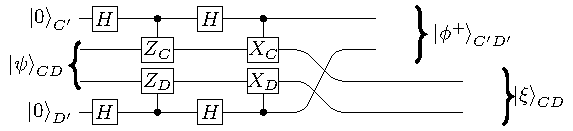
\includegraphics[scale=1.2]{giraffics/CHSH-swap.pdf}
\end{center}
Where a direct calculation using the above listed properties of $Z_*, X_*$ gives the right hand side.
This above example was described by Mayers and Yao in \cite{mayers2003self}, where they also give the first characterization of self-testing.

\section{Connections to Non-Local Games}
One might note the implicit connection between the formulation of a self-test and the underlying correlations given by some optimal strategy to a non-local game.
In particular, work by Slofstra in \cite{slofstra2011lower} associates to each XOR game $\mcG$ a game $C^*$-algebra where optimal strategies winning $\mcG$ correspond to representations of the game $C^*$-algebra.
The same paper also generalized the CHSH game to higher dimensions and provided similar self-testing protocols as above for higher dimensional maximally entangled qudits.

\section{Extensions of Self-Testing}
We remarked earlier that it is necessary for the self-testing protocol to be multipartite, as in the unipartite case a lab running an exceptionally powerful simulator can convince any tester of unipartite quantum operations.
In motivating self-testing as a protocol, however, we wished to be able to prove without examining an experimental setup,
that the experiment must be doing something quantum.
It is then of use to be able to verify that an experimenter implementing a quantum circuit (perhaps through a sequence of gates) has correctly done so.

Work done in \cite{magniez2006self} shows that this is indeed possible.
To do so, Carl and David must be given access to the same physical implementation of the gate.
For experimental setups, this is not too restrictive of an assumption.
Suppose then we wish to show that the implementation of some single qubit gate $G$ is experimentally realized by some gate $G'$.
The protocol is as follows:

In the first step, we perform the Mayers-Yao self-test on some input state $\ket{\psi}$ to prove that it is in fact the maximally entangled state. This verifies both the initial state and the measurements used.

Next, Carl and David both apply the gate $G$ to their halves of the EPR pair. The Mayers-Yao self-test is then done on this state which then ensures that it is indeed a unitary gate on the support of $\ket{\phi^+}$.

Finally, a check that the Mayers-Yao measurements on $G'_C\otimes \one_D \ket{\psi}$ reproduces the same outcomes
as the theoretical $G_C\otimes \one_D\ket{\phi^+}$.

This protocol can be extended to $n$-qubit gates by having Carl and David share $n$ EPR pairs.
Briefly, the first step remains the same, and the second and third simply corresponds to performing $n$ Mayers-Yao self-tests on each of the wires simultaneously.

We remark that the ability then to self-test gates then allows one to self-test the implementation of a circuit by simply verifying that each individual gate is implemented correctly.

% \section{Conclusion and Outlook}
% \label{sec:outlook}
% \lipsum[1-2]

% \subsubsection*{Acknowledgments}

% Identification of funding sources and other support, and thanks to individuals and groups that assisted in the research and the preparation of the work should be included in an acknowledgment section, which is placed just before the reference section in your document \cite{acmart}.

% %%% ===============================================================================
% %%% Bibliography
% %%% ===============================================================================

% In the bibliography, use \texttt{\textbackslash textsuperscript} for \enquote{st}, \enquote{nd}, \ldots:
% E.g., \enquote{The 2\textsuperscript{nd} conference on examples}.
% When you use \href{https://www.jabref.org}{JabRef}, you can use the clean up command to achieve that.
% See \url{https://help.jabref.org/en/CleanupEntries} for an overview of the cleanup functionality.

\renewcommand{\bibsection}{\section*{References}} % requried for natbib to have "References" printed and as section*, not chapter*
% Use natbib compatbile splncs04nat style.
% It does provide all features of splncs04.bst, but is developed in a clean way.
% Source: https://github.com/tpavlic/splncs04nat
\bibliographystyle{splncs04nat}
\begingroup
  \microtypecontext{expansion=sloppy}
  \small % ensure correct font size for the bibliography
  \bibliography{paper}
\endgroup

% Enfore empty line after bibliography
\ \\
%
\noindent
% All links were last followed on October 5, 2020.

%%% ===============================================================================
%\appendix
%\addcontentsline{toc}{chapter}{APPENDICES}

%\listoffigures
%\listoftables
%%% ===============================================================================

%%% ===============================================================================
%\section{My first appendix}\label{sec:appendix1}
%%% ===============================================================================
\end{document}
